\documentclass{article}
\usepackage[utf8]{inputenc}
\usepackage{fullpage}
\usepackage{amsmath}
\usepackage{hyperref}
\usepackage{amssymb}
\usepackage[most]{tcolorbox}
\usepackage{empheq}
\usepackage{mhchem}
\usepackage{braket}
\usepackage{graphicx}

\newtcbox{\mymath}[1][]{%
    nobeforeafter, math upper, tcbox raise base,
    enhanced, colframe=black!30!black,
    colback=black!30, boxrule=1pt,
    #1}
    
\title{Computational HW 4}
\author{Marcus DuPont}
\date{\today}

\begin{document}

\maketitle

\begin{enumerate}
    \item {\textbf{Newman 8.18}
    Chemical reactions  are described by the following differential equations
    \begin{align*}
        \frac{dx}{dt} &= 1 + ax^2y - (b+1)x & \frac{dy}{dt} &= bx -ax^2y
    \end{align*}
    The solutions to such equations are described below.
    \begin{figure}[h!]
        \centering
        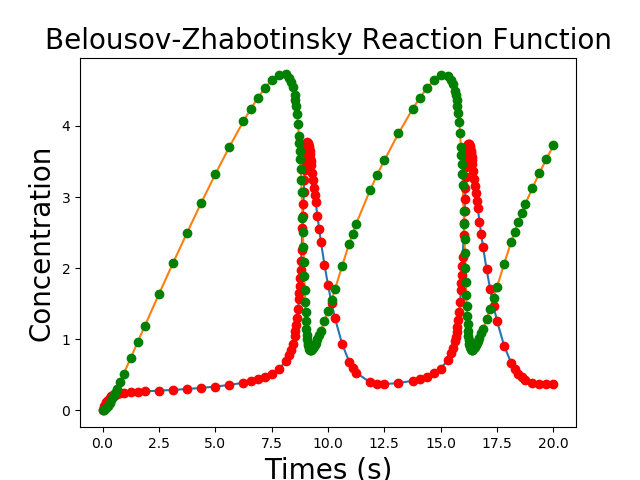
\includegraphics[width=\textwidth]{BZ.png}
        \caption{Plot of the oscillating chemical concentrations described by the Belousov-Zhabotinsky Differential Equation.}
        \label{fig: bk}
    \end{figure}
    }
    \item {\textbf{Black Hole Merger}
    The black hole equation of motion in the presence of the dynamical friction is shown:
    \begin{equation*}
        \partial_{tt}\pmb{r_{BH}} = - \frac{GM_{BH}}{4r_{BH}^3}\pmb{r_{BH}} + \pmb{\dot{v_{DF}}},
    \end{equation*}
    where $\pmb{\dot{v_{DF}}}$ is the dynamical friction force driving the decay of the black hole binary orbit.
    \begin{enumerate}
        \item{From trial and error, one can build a function where the $\delta$ value is defined by the user.
        I guessed a value of $\delta = 10^{-6}$.}
        \item{
        \begin{figure}[h!]
            \centering
            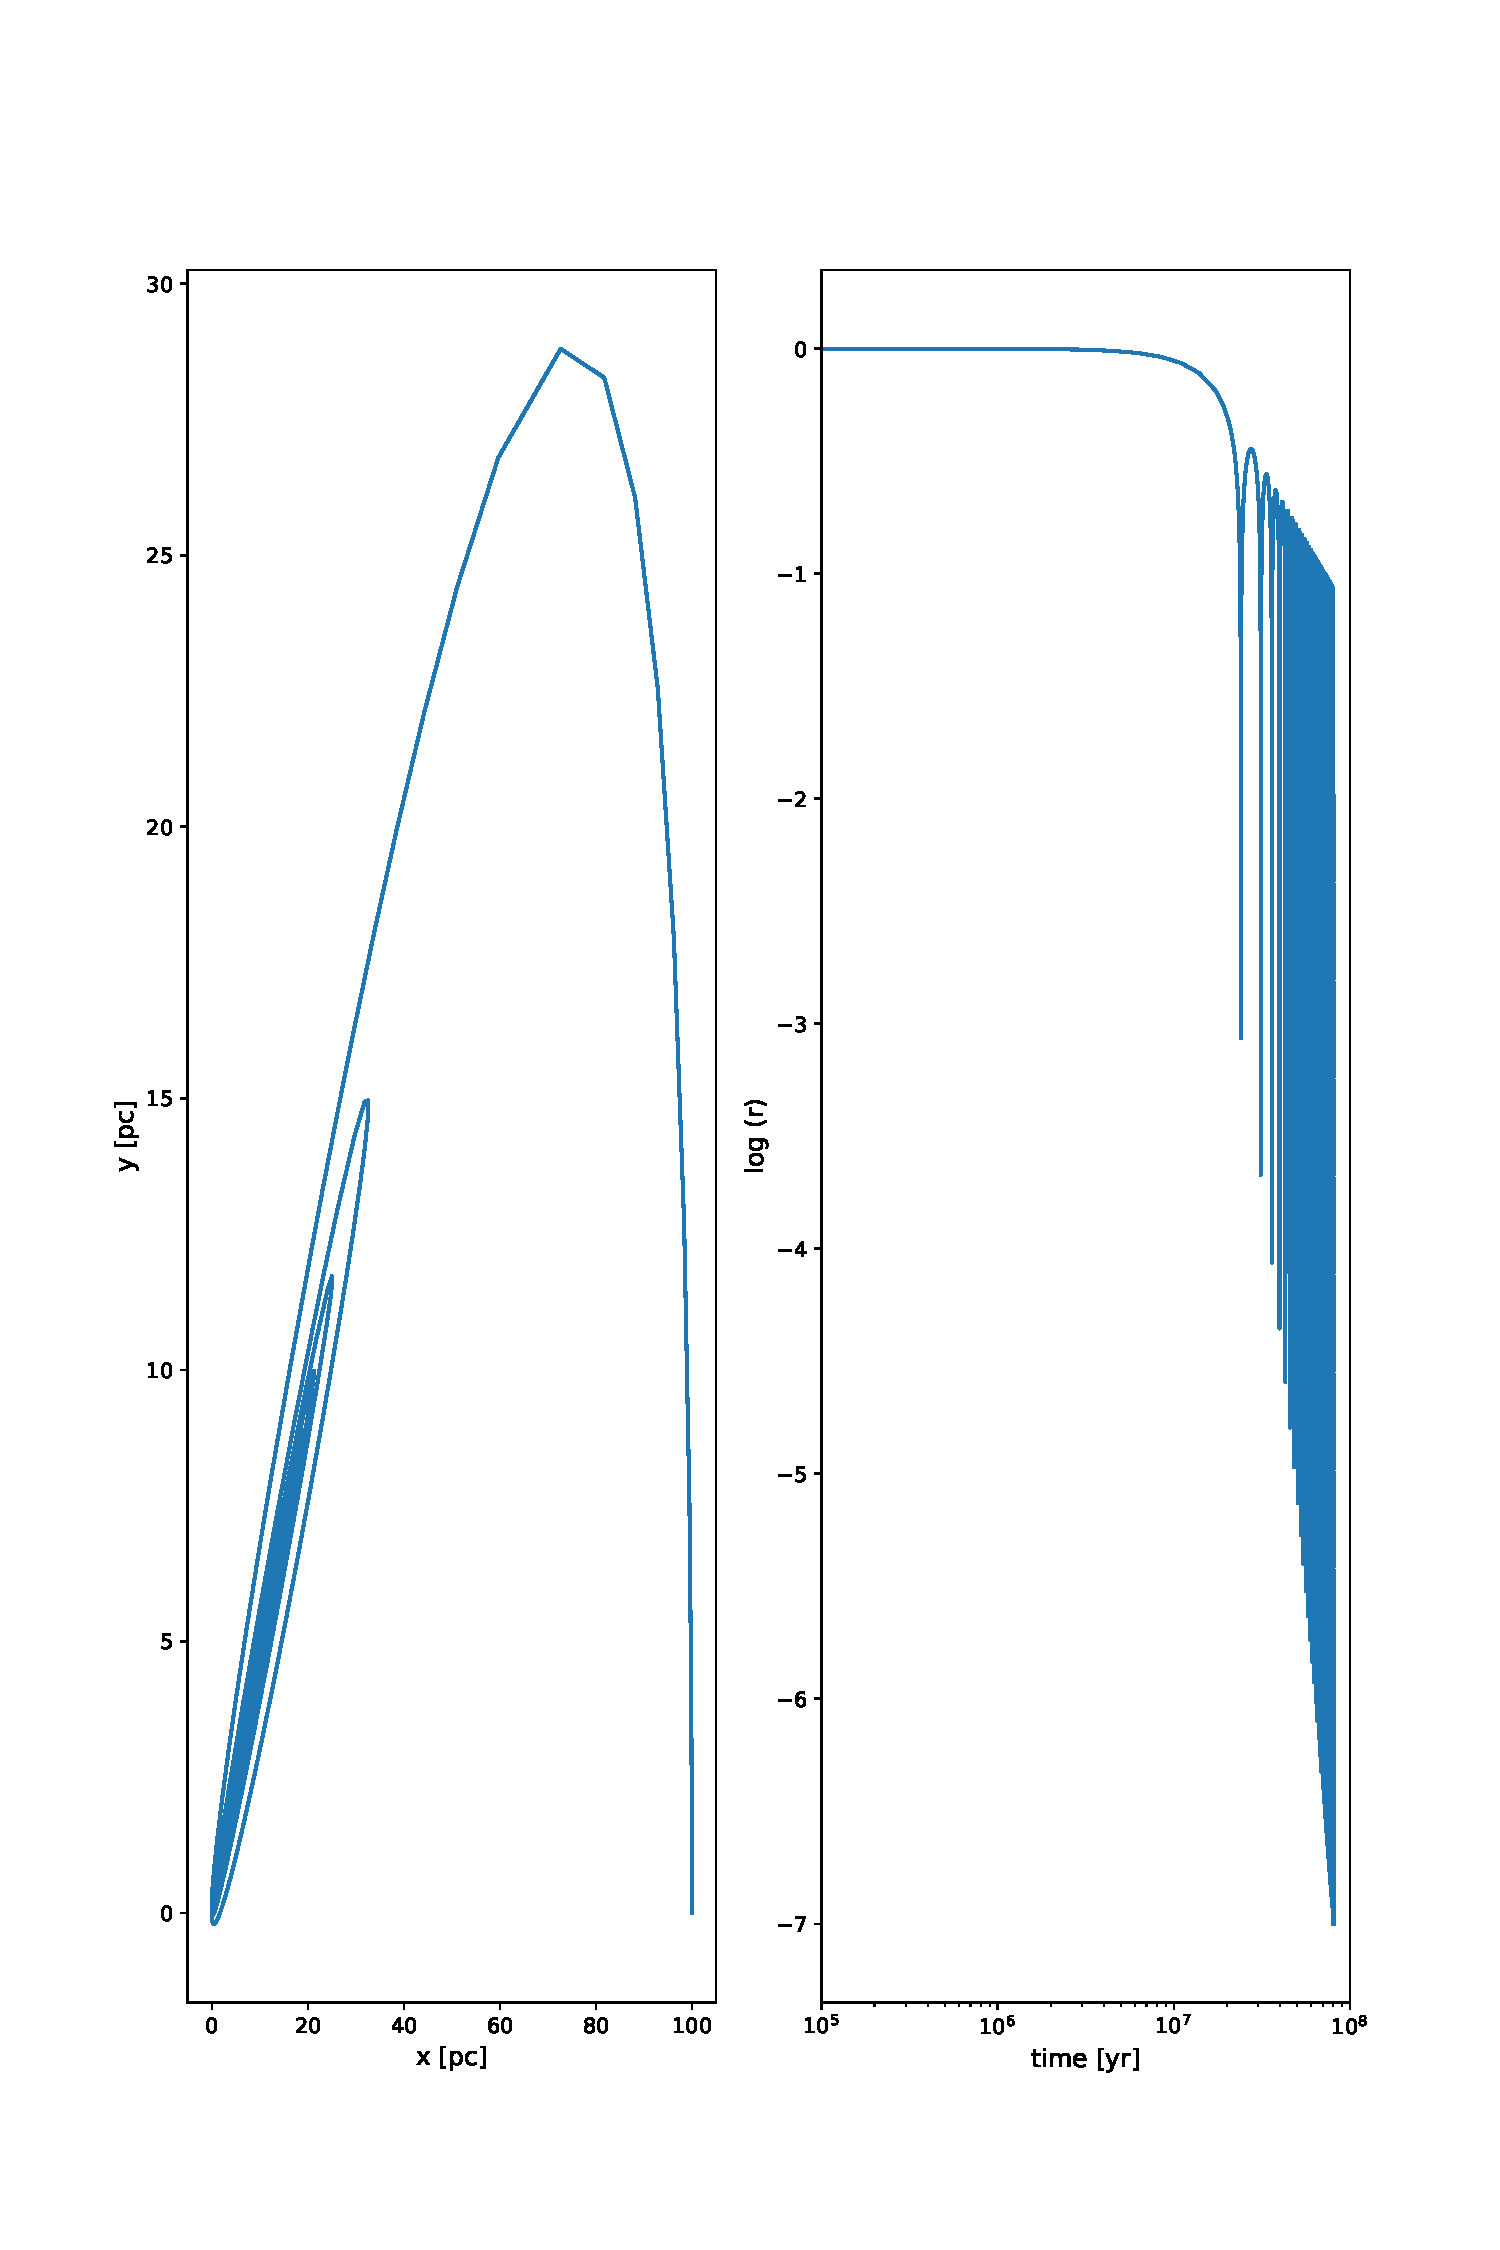
\includegraphics[width=\textwidth, height=15cm]{Bh_trajectory_xy.pdf}
            \caption{The left plot shows the black holes trajectory starting from coordinates (1,0). The left plot shows the oscillatory behavior of the black hole as it approaches the Swartzschild radius $r_s$. }
            \label{fig:my_label}
        \end{figure}
        }
        \item{The recursion depth limited the calculation, but the physics behind the Swartzschild radius falling. The ratio $B/A$ is governed by the velocity dispersion, stellar density, and black hole mass. If I were to make a guess, the ratio $B/A$ governs the amount of angular momentum within the system. If the ratio is small, the black holes will converge faster because there is less angular momentum stolen from their orbits. The ratio effusively follows a power law in terms of the black hole merging time}
        \item{The initial velocity of the black holes enforce the semi-major axis of the orbits. The initial black hole energy describes where it lies within the potential well of the other orbiting body. The higher up in the potential well, the larger the semi-major axis. Aside from that, the ratio $B/A$ describes the relative fraction of velocity dispersion and stellar density, so the amount of stars present versus the spread of their velocities will perturb the black hole orbits enough to slow their radial decay or if the ratio is too small, the black holes will merge much sooner.}
    \end{enumerate}
    }
\end{enumerate}

\end{document}
